\section{How strongly does the char-removal assumption affect time?}\label{sec:removal}
The local surface law charges an effective energy $L_c$ for each kilogram of
char removed. The earlier energy inventory shows why this coefficient matters.
To vary it in isolation, we keep the gas at 2504~K and 800~psi, the nominal
film coefficient at 1000~W/(m$^2$~K), and the same kinetics, char yield,
case geometry and casing response. We solve again with half and twice the
inherited $35$~MJ/kg. These values bracket an assumption. No Iris sample
measurement establishes a probability distribution or physical bounds.

\begin{center}\begin{tabular}{lrrr}\toprule
&\multicolumn{3}{c}{Independent time from exposure to liner loss [s]}\\
Motor & 17.5 MJ/kg & 35 MJ/kg & 70 MJ/kg\\\midrule
Sustainer Al & 71.8 & 110.5 & 184.7 \\
Sustainer CF & 64.9 & 104.3 & 179.0 \\
Booster Al & 95.9 & 147.6 & 246.7 \\
Booster CF & 85.4 & 137.9 & 237.7 \\
\bottomrule\end{tabular}\end{center}
\begin{figure}[H]\centering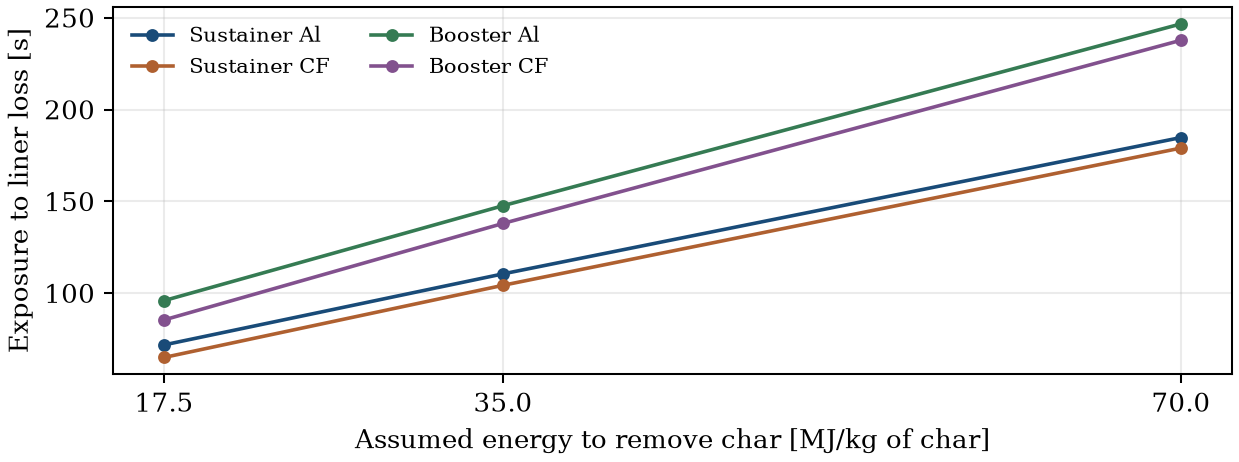
\includegraphics[width=.96\textwidth]{../analysis/evolving_removal_cost.png}
\caption{The symbols are separate finite-volume simulations. Lines join the
sampled settings. The Al and CF backings evolve during every case.}
\end{figure}

An increased removal cost leaves less of the incoming heat available to
consume char at the surface. Temperature, heat transfer from the gas,
and the available char also change during each run. The time therefore need
not scale in direct proportion to $L_c$. The time-step and radial mesh checks
use separate refinements. Each published value passes the time, thickness and
mass/energy checks, and has a separate nodal finite-element comparison.

A useful calibration would measure the applied heat flux, time-resolved
surface recession and remaining char for a specimen of the actual liner.
A residual thickness alone cannot separate excessive heating from an
underestimated removal cost. The film study varies the heat load separately.
\clearpage
